\chapter{Control de PAMH basado en aprendizaje reforzado}
\label{ch:ControlPAMH}

Para obtener un modelo controlador de una planta como el péndulo amortiguado de motor con hélice, es necesario definir el modelo de RL a utilizar, el plan de entrenamiento del modelo y la función de recompensa que conduzca al comportamiento deseado del agente.

\section{Selección de modelos de RL}

En primera instancia se realiza una investigación biblográfica respecto a los métodos de RL comunmente utilizados para el control de entornos o sistemas similares a la planta PAMH, al igual que una búsqueda de repositorios o publicaciones realizadas para cada método de RL encontrado, de manera que cada uno de los métodos contara con un respaldo para la evaluación de los criterios seleccionados para la matriz de Pugh, mostrada la tabla \ref{tab:MatrizPugh}.

\begin{table}[h]
\centering
\caption{Matriz de Pugh de los métodos de RL cantidadatos.}
\begin{tabular}{lccccc}
\hline
\multicolumn{1}{|c|}{\multirow{2}{*}{\textbf{Criterios}}} &
  \multicolumn{1}{c|}{\multirow{2}{*}{\textbf{Peso}}} &
  \multicolumn{4}{c|}{\textbf{Alternativas}} \\ \cline{3-6} 
\multicolumn{1}{|c|}{} &
  \multicolumn{1}{c|}{} &
  \multicolumn{1}{l|}{\textbf{DQN}} &
  \multicolumn{1}{l|}{\textbf{PPO}} &
  \multicolumn{1}{l|}{\textbf{DDPG}} &
  \multicolumn{1}{l|}{\textbf{SAC}} \\ \hline
\multicolumn{1}{|l|}{\begin{tabular}[c]{@{}l@{}}Fiabilidad de control del PAMH\end{tabular}} &
  \multicolumn{1}{c|}{4} &
  \multicolumn{1}{c|}{0} &
  \multicolumn{1}{c|}{+1} &
  \multicolumn{1}{c|}{+1} &
  \multicolumn{1}{c|}{+1} \\ \hline
\multicolumn{1}{|l|}{Recursos computacionales} &
  \multicolumn{1}{c|}{3,5} &
  \multicolumn{1}{c|}{+1} &
  \multicolumn{1}{c|}{+1} &
  \multicolumn{1}{c|}{0} &
  \multicolumn{1}{c|}{-1} \\ \hline
\multicolumn{1}{|l|}{Tiempo de desarrollo} &
  \multicolumn{1}{c|}{3} &
  \multicolumn{1}{c|}{+1} &
  \multicolumn{1}{c|}{+1} &
  \multicolumn{1}{c|}{0} &
  \multicolumn{1}{c|}{0} \\ \hline
\multicolumn{1}{|l|}{Código existente} &
  \multicolumn{1}{c|}{2,5} &
  \multicolumn{1}{c|}{+1} &
  \multicolumn{1}{c|}{+1} &
  \multicolumn{1}{c|}{0} &
  \multicolumn{1}{c|}{0} \\ \hline
\multicolumn{1}{|l|}{Optimización} &
  \multicolumn{1}{c|}{2} &
  \multicolumn{1}{c|}{+1} &
  \multicolumn{1}{c|}{+1} &
  \multicolumn{1}{c|}{0} &
  \multicolumn{1}{c|}{0} \\ \hline
\multicolumn{1}{|l|}{Tiempo de entrenamiento} &
  \multicolumn{1}{c|}{1,5} &
  \multicolumn{1}{c|}{-1} &
  \multicolumn{1}{c|}{+1} &
  \multicolumn{1}{c|}{0} &
  \multicolumn{1}{c|}{+1} \\ \hline
\multicolumn{1}{|l|}{Innovación} &
  \multicolumn{1}{c|}{1} &
  \multicolumn{1}{c|}{-1} &
  \multicolumn{1}{c|}{0} &
  \multicolumn{1}{c|}{+1} &
  \multicolumn{1}{c|}{+1} \\ \hline
 &
  \multicolumn{1}{l}{} &
  \multicolumn{1}{l}{} &
  \multicolumn{1}{l}{} &
  \multicolumn{1}{l}{} \\ \cline{1-1} \cline{3-6} 
\multicolumn{1}{|l|}{\textbf{Suma general}} &
  \multicolumn{1}{c|}{} &
  \multicolumn{1}{c|}{8,5} &
  \multicolumn{1}{c|}{16,5} &
  \multicolumn{1}{c|}{5,0} &
  \multicolumn{1}{c|}{3.0} \\ \cline{1-1} \cline{3-6} 
\multicolumn{1}{|l|}{\textbf{Ranking}} &
  \multicolumn{1}{c|}{} &
  \multicolumn{1}{c|}{2"o} &
  \multicolumn{1}{c|}{1"o} &
  \multicolumn{1}{c|}{3"o} &
  \multicolumn{1}{c|}{4"o} \\ \cline{1-1} \cline{3-6} 
\end{tabular}
\label{tab:MatrizPugh}
\end{table}

La revisión de material respecto al algoritmo DQN se encuentra en el documento base del método \cite{DQNbase} publicado en el año $2013$ y los criterios o consideraciones importantes al respecto se encuentran en \cite{DQNexplained} y \cite{PytorchDQN}, como el problema de convergencia con espacios de acciones continuos \cite{ForoDQN}. En resumen, el método DQN cuenta con amplio respaldo de ejemplos de implementación en RL y presenta entrenamientos con resultados eficientes para espacios de acciones discretos y soluciones discretizadas.

En cuanto al método PPO, se consultó el documento base del método \cite{PPObase} publicado en el año $2017$ y de igual forma, repositorios y artículos sobre sus casos de aplicación, donde se demuestra su eficiencia al trabajar tanto con espacios de acciones discretos como continuos \cite{PPOyu} y \cite{PPOcoding2}.

El caso del método gradiente de política determinista profunda (DDPG, por sus siglas en inglés) publicado en el año $2019$, responde a una solución de los problemas del DQN con espacios continuos, en ocaciones conocido como DQN para espacios continuos. El algoritmo utiliza lógica del conocido DQL e implementaciones de políticas de igual forma \cite{DDPGbase}.

También se tiene el método actor-crítico blando (SAC, por sus siglas en inglés) publicado en el año $2018$, un algoritmo basado en RL de máxima entropía, pues el componente actor busca maximizar la recompensa esperada junto con la entropía, por lo que la convergencia a un comportamiento deseado es caracterizado por pasos ``suaves'' en lugar de saltos abruptos en acciones \cite{SACbase}.

El factor del recurso computacional requerido define el tiempo de entrenamiento o en algunos casos, la posibilidad de implementación del método. El DQN dispone de amplio repositorio de ejemplos, pero se trata del método de mayor antiguedad, por lo que no presenta el mismo enfoque de disminución de tiempos a costo de la capacidad de cálculo como si lo hicieron DDPG y SAC \cite{DDPGbase} \cite{SACbase}.

Por otro lado, los métodos DDPG y SAC al ser nuevos en comparación con los otros, no cuentan con el amplio registro de repositorios de implementación y pasos extra de optimización, mientras si cuentan con extensos algoritmos de funcionamiento, por lo que su tiempo de desarrollo se ve afectado.

El método PPO presenta las mejores cualidades para ser utilizado como algoritmo entrenador de un controlador para el entorno PAMH, descrito en el capítulo \ref{ch:teoria}. Como segunda posición se tiene el método DQN, por lo que se puede seleccionar de acuerdo con lo recomendado en las publicaciones referentes a su uso con discretización del espacio de acciones continuo.

\section{Preparación de entornos virtuales}

Dada la complejidad de los métodos de RL utilizados, el primer paso consiste en una implementación con entornos virtuales conocidos. La plataforma Gymnasium de Farama Fundation \cite{Gymnasium} ofrece una colección de entornos de código abierto disponibles para experimentación con estrategias de control. Los entornos consisten en simulaciones físicas de entornos particulares como péndulos simples y dobles, con actuadores y un conjunto de acciones predefinidas \cite{Gymnasium}.  

Luego del estudio de los algoritmos pertinentes para la aplicación del RL mediante PPO y DQN \cite{PPObase} \cite{DQNbase}, se aplican ajustes para funcionar, en primera fase, con entornos de acciones discretas, como es el caso del problema de control del péndulo invertido (\textit{CartPole}) \cite{Gymnasium}.

El segundo paso es adaptar el código para trabajar con entornos con características y mediciones de valores continuos. Como caso de estudio se usa el control del otro péndulo invertido (\textit{Pendulum}), en el cual se realizan las primeras pruebas de ajuste de ángulo objetivo, dado que el objetivo base del entorno es mantener el ángulo superior estático ($0^o$). Por lo tanto, el primer ajuste al método fue la implementación del error de ángulo:
\begin{equation}
E_{\theta} = |\theta - \theta_{objetivo}|
\label{ecu:errorangular}
\end{equation}
en lugar de únicamente el componente $\theta$ del péndulo en su función de recompensas, heredada del código base de Gymnasium \cite{Gymnasium}.

Para facilidad de acoplamiento de los modelos experimentales anteriores al caso concreto de PAMH, se adapta el modelo mimetizador del proyecto previo \cite{JorgeBrenes} a una interfaz de tipo Gymnasium, de manera que el modelo imitador del PAMH trabaje de forma similar a los modelos disponibles de RL que se usan en Gymnasium.

En las mediciones u observaciones al entorno simulado o real PAMH, hay un único valor observable: el ángulo del péndulo de la planta. Se adicionan parámetros de información para el procesamiento de la red neuronal para complementar el estado con aproximaciones de la primera derivada (como velocidad angular) de la forma:
\begin{equation}
\dot{\theta} = \theta_t - \theta_{t-1}
\end{equation}
y la segunda derivada (como aceleración):
\begin{equation}
\ddot{\theta} = \dot{\theta}_t - \dot{\theta}_{t-1}
\end{equation}
ambos casos basados en las diferencias entre los valores medidos en la actual iteracion $t$ y la anterior iteración $t-1$. 

Se agrega además a las observaciones el valor del ángulo objetivo $\theta_{objetivo}$, con la intención de que la red pueda aprender a inferir diferencias de comportamiento de la planta, dependientes del objetivo que esta deba alcanzar; pues no es lo mismo controlar para llegar a $10^o$ que a $90^o$. Por lo tanto, el vector utilizado de observación de la planta es:

\begin{equation}
obs_n = [\theta \, ,\quad \dot{\theta} \, ,\quad \ddot{\theta} \, ,\quad \theta_{objetivo}]
\label{ecu:observation}
\end{equation}

lo que corresponde al mapeo $\phi(s)$ de una dimensión a cuatro dimensiones, propuesto en este trabajo para cumplir la función introducida de forma general en la ecuación (\ref{ecu:accionDQN}).

\section{Parametrización de los modelos}

Uno de los puntos clave del trabajo realizado es el diseño de la función de recompensa enfocada en guiar al comportamiento deseado.

De igual forma, se presentan a continuación las configuraciones de los dos métodos seleccionados DQN y PPO.

\subsection{Función de recompensa}

La función de recompensa condiciona el comportamiento del agente por su relación directa con las características deseadas respecto a su comportamiento en el entorno.

Con base en los fundamentos relacionados a la planta PAMH, el problema definido para el agente es mantener un ángulo constante, indicado con anterioridad, además de alcanzar una velocidad angular baja, cuando se alcance el ángulo final.

Por lo tanto, se propone una ecuación que recompense alcanzar el ángulo deseado y caso contrario, castigar un ángulo diferente al deseado y una velocidad angular alta, pues este último indicaría que no se estabiliza el péndulo. La función propuesta se muestra en el algoritmo \ref{alg:reward}.

\begin{algorithm}[hh]
\caption{Función de recompensa}\label{alg:reward}
\begin{algorithmic}[1]
\State Recibe los componentes de la observación $\theta$, $\dot{\theta}$.
\State Recibe la señal de acción $PWM$ anterior $a_{t-1}$.
\State Recibe el ángulo objetivo $\theta_{objetivo}$.
\State Asegura el valor $\theta$ en radianes y en el rango $[-\pi,\pi]$.
\State Cálculo del error: 
\[E_{\theta} = |\theta - \theta_{objetivo}|\]
\State Potenciar y escalar el comportamiento no deseado con el costo por error angular $C_\theta$ y el costo por velocidad angular $C_{\dot{\theta}}$:
\[C_{\theta} = \theta^2_{error}\]
\[C_{\dot{\theta}} = 100 \cdot \dot{\theta}^2\]
\State Recompensa por comportamiento deseado:
\[R_{\theta} = 2 \cdot \left( e^{-C_{\theta}/\sigma_r} \, (1 - |C_{\dot{\theta}}|)\right)\]
\State Recompensa y castigo por señal de acción deseada:
\[E_{a_{t-1}} = \left\{ \begin{array}{ll}
0 & \mbox{para acción $0<|a_{t-1}|<0.25$} \\
20^{|a_{t-1} - 0.25|} & \mbox{para el resto de $a_{t-1}$}
\end{array}
\right.\]
\State La señal de recompensa resultante:
\[R = \min \left[-C_{\theta}, \,\, -E_{a_{t-1}}\right] + R_{\theta}\]
\end{algorithmic}
\end{algorithm}

En este caso la función de recompensa se centra en dos de las cuatro observaciones del entorno: el ángulo del péndulo $\theta$ y la velocidad ángular $\dot{\theta}$. El objetivo de este caso es alcanzar el ángulo objetivo y que el péndulo permanezca estático allí. Por lo tanto, primero se verifica la escala del ángulo medido $\theta$ para evitar problemas de precisión por redundancia de ángulos fuera de rango $[-\pi, \pi]$. Luego se calcula el error angular que es potenciado al cuadrado para dar mayor castigo a los valores lejanos al $\theta_{objetivo}$. La baja magnitud de $\dot{\theta}$ requiere aumentar cien veces su valor para afectar la comparación con el ángulo y potenciarla para mayor castigo por movimientos rápidos, lo que se determina experimentalmente.

El valor de $R_{\theta}$ busca recompensar la cercanía con el objetivo, pero solo al máximo ($R_{\theta}=2$) si la velocidad $\dot{\theta}$ mantiene un valor cercano a cero, aproximación a péndulo estático. 

El componente $E_{a_{t-1}}$ es el error por la acción anterior que produjo la observación $obs_n$ y castiga la generación de señal PWM por encima del $0.25$, valor elevado para la planta real, por lo que se debe evitar. Si la señal de acción se mantiene en el rango con límite inferior $0,0$ y límite superior $0.25$, no hay castigo.

La salida del algoritmo selecciona el mayor castigo entre el $C_{\theta}$ y $E_{a_{t-1}}$; si la señal de acción se encuentra en rango, la recompensa solo será el error del ángulo con la recompensa por cercanía con el objetivo.

La figura \ref{fig:rewfunc} muestra la función de recompensa con $\theta_{objetivo} = 45^o$ con un rango de $-120^o$ a $120^o$ y mayor detalle de la curva alrededor del objetivo se ilustra en la figura \ref{fig:rewfunccampana}. Como se observa, a mayor distancia con el objetivo, mayor castigo, como el caso de un $\theta \approx 100^o$ con una recompensa de aproximadamente $-1$ unidades, mientras el castigo tiende a cero si se acerca al $\theta_{objetivo}$, punto en que se influye el componente $R_{\theta}$, afectando un caso de $\theta \approx 43^o$ con recompensa de $1.5$ unidades aproximadamente.
\begin{figure}[hh]
	\centering
	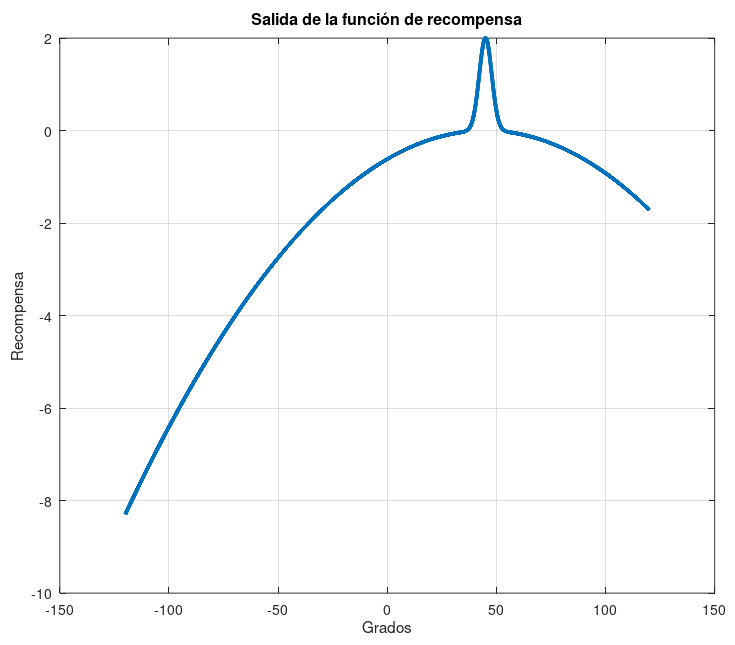
\includegraphics[scale=0.4]{fig/new/Rewardfunc.png}
	\caption{Función de recompensa con $\theta_{objetivo}=45^o$.}
	\label{fig:rewfunc}
\end{figure}

\begin{figure}[hh]
	\centering
	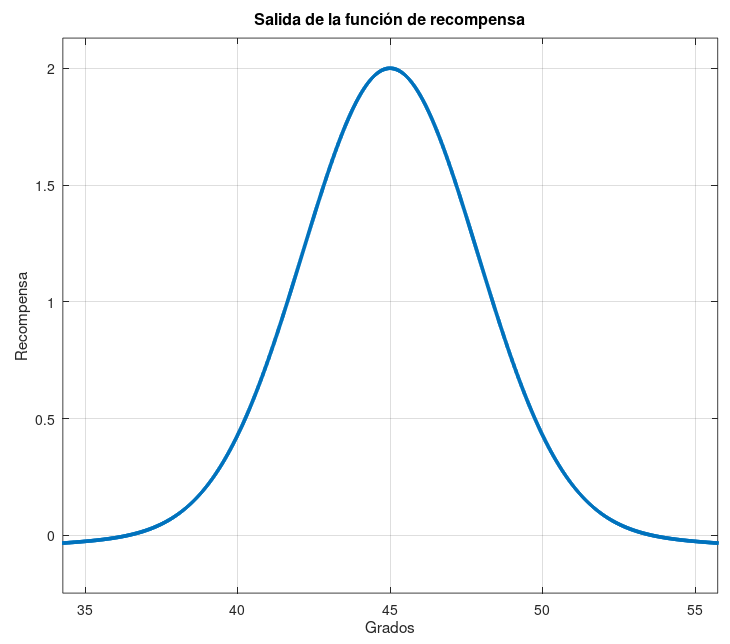
\includegraphics[scale=0.4]{fig/new/Rewardfunccampana.png}
	\caption{$\theta_{correcto}$ con $\theta_{objetivo}=45^o$.}
	\label{fig:rewfunccampana}
\end{figure}
 
Cabe resaltar que para la definición del último punto de la función de recompensas expuesta, se requirió de experimentación con numerosos entrenamientos de los modelos, pues un cambio como la aplicación de una resta lineal
\begin{equation}
R = -C_{\theta} -E_{a_{t-1}} + R_{\theta}
\end{equation}
o prescindir del componente $E_{a_{t-1}}$, da libertad al modelo para explorar sus límites de acción. La aplicación de la técnica de moldear la recompensa (\textit{reward shaping}), impactan sensiblemente el desempeño del agente, en este caso seleccionando la opción del algoritmo \ref{alg:reward} por mantener el nivel del resultado del proceso de entrenamiento estable \cite{RewardShaping}.
 
\subsection{Estructura de las RNA en DQN y PPO}

La estructura general de las RNA en ambos modelos utiliza una capa de entrada definida por el número de observaciones del entorno, anteriormente definido como $obs_n$ en la ecuación (\ref{ecu:observation}), una capa de salida definida por el número de acciones posibles por método, descritos en las siguiente secciones, y un conjunto de tres capas densas (completamente conectadas) con número de neuronas $64$, $128$, $64$, respectivamente, para requerir un aumento de dimensión y acceso a procesamientos más complejos en la RNA, esto definido para cada método \cite{DataScience}.

Como capas de activación, se utiliza ReLU (\textit{rectified linear unit}) por la condición del espacio de acciones base del entorno: valores de PWM en el rango de $0.0$ a $1.0$, de manera que los valores positivos sean recibidos de manera lineal y los negativos ignorados \cite{DataScience}.
 
 
\subsection{DQN}

\subsubsection{Discretización}

Como se mencionó en el capítulo \ref{ch:teoria}, el método DQN se utiliza en el control de sistemas; sin embargo, la literatura indica que DQN tiene problemas en el caso de entornos con espacios de acciones continuos \cite{ForoDQN}.

Por lo tanto, se discretizan las acciones del entorno, que oficialmente trabaja en el rango de $0.0$ a $1.0$ de PWM. De acuerdo con \cite{JorgeBrenes}, el límite superior del espacio de acciones se fija por seguridad en $0.25$ de PWM para cuidar la integridad del equipo real, por lo que se respetó en las pruebas virtuales, además de que la RNAM no conoce el comportamiento de la planta real fuera de ese rango.

Se selecciona una cantidad de $10$ posibles acciones discretas, producto de la experimentación, lo cual responde a la función:
\begin{equation}
a_d = \left\lfloor 36 \cdot a \right\rfloor
\end{equation}
para el proceso de discretización y la función:
\begin{equation}
a = \frac{a_d}{36}
\end{equation}
para el proceso de desdiscretización. Esto deja un espacio de acciones discretas mostradas en la tabla \ref{tab:accionesdis}.
\begin{table}[h]
\centering
\caption{Equivalencia de valores continuos y discretos seleccionados para el método DQN.}
\label{tab:accionesdis}
\begin{tabular}{|l|cccccccccc|}
\hline
\textbf{Tipo}         & \multicolumn{10}{c|}{\textbf{Acción equivalente}}                                                                                                                                                                                                               \\ \hline
Continua (aproximada) & \multicolumn{1}{c|}{0.0} & \multicolumn{1}{c|}{0.03} & \multicolumn{1}{c|}{0.06} & \multicolumn{1}{c|}{0.08} & \multicolumn{1}{c|}{0.11} & \multicolumn{1}{c|}{0.14} & \multicolumn{1}{c|}{0.17} & \multicolumn{1}{c|}{0.19} & \multicolumn{1}{c|}{0.22} & 0.25 \\ \hline
Discreta              & \multicolumn{1}{c|}{0}   & \multicolumn{1}{c|}{1}    & \multicolumn{1}{c|}{2}    & \multicolumn{1}{c|}{3}    & \multicolumn{1}{c|}{4}    & \multicolumn{1}{c|}{5}    & \multicolumn{1}{c|}{6}    & \multicolumn{1}{c|}{7}    & \multicolumn{1}{c|}{8}    & 9    \\ \hline
\end{tabular}
\end{table}

\subsubsection{RNA para DQN}

Tomando la base ya expuesta, la RNA utilizada para el método DQN parte de las estructuras encontradas en repositorios como \cite{PytorchDQN}, utilizando $128$ neuronas en la capa densa central, a la que se le suman una capa densa previa y una capa densa posterior, ambas de $64$ neuronas para el aumento y disminución de la dimensionalidad. Por último, se acopla la capa de salida con las $10$ posibles salidas de valores Q mencionadas. El resultado como tal se muestra en la figura \ref{fig:RNAparaDQN}, de manera que se obtiene un vector $Q_n$ con los valores Q para cada posible acción.

\begin{figure}[hh]
	\centering
	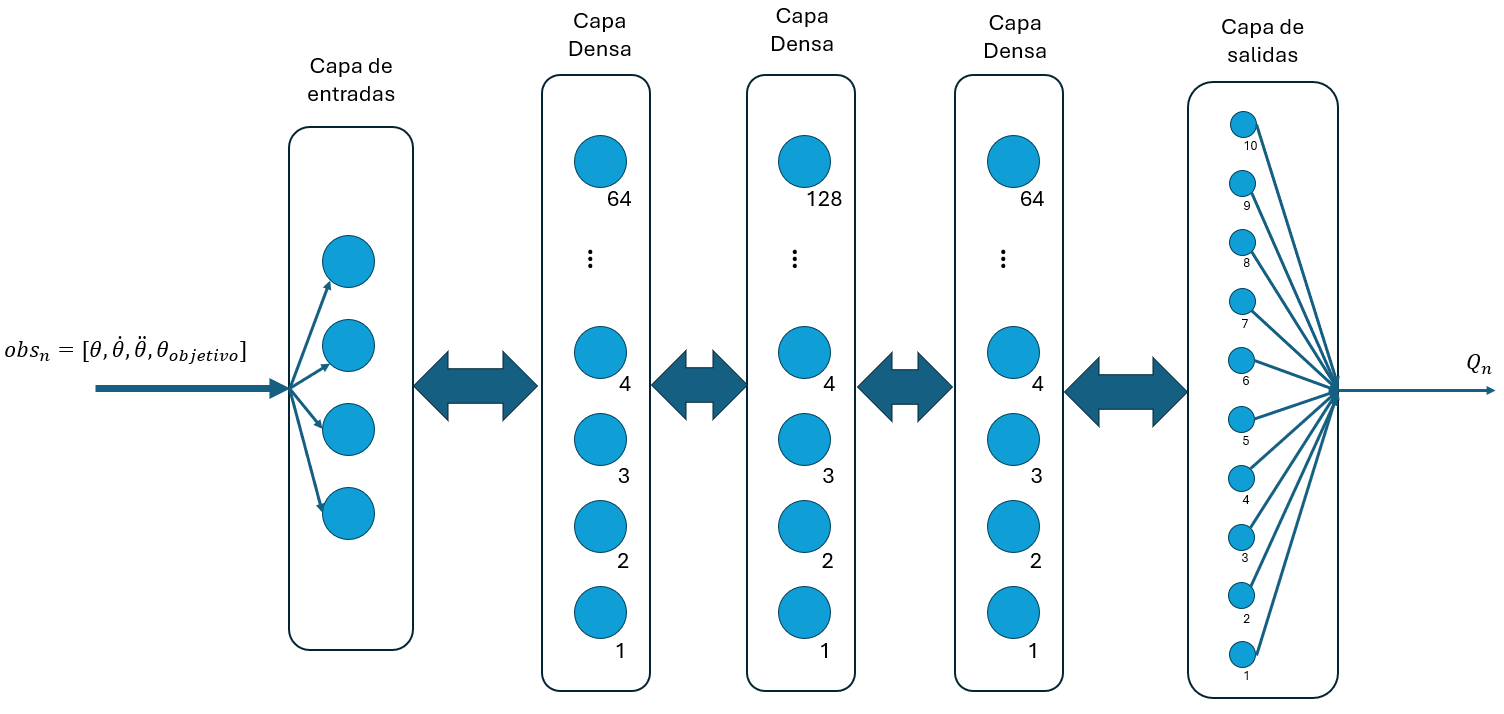
\includegraphics[scale=0.38]{fig/new/RNADQN.png}
	\caption{Estructura de la RNA utilizada en el método DQN.}
	\label{fig:RNAparaDQN}
\end{figure}

\subsubsection{Plan de entrenamiento}

El esquema original de entrenamiento de DQN se modifica en la selección de la acción; utilizando avaro-$\varepsilon$, la etapa de exploración implica la generación de un valor de ruido $n_{ruido}$ que es sumado a la acción discreta dictada por la RNA que aproxima (\ref{ecu:accionDQN}), obteniendo:
\begin{equation}
a_{t_{ruido}} = a_t + n_{ruido}
\end{equation}
donde $n_{ruido}$ varía en principio en un rango con magnitud máxima de $6$ y mínima $0$. Luego al alcanzar la mitad del tiempo de entrenamiento, la magnitud máxima del ruido se reduce a $4$ y luego de tres cuartos del tiempo se reduce a $2$. Por lo tanto, el avaro-$\varepsilon$ reduce las probabilidades de adición de ruido y al mismo tiempo la magnitud del ruido $n_{ruido}$ se diminuye con el avance del entrenamiento, pasando a un método de explotación de lo aprendido.

\subsection{PPO}

\subsubsection{RNA para PPO}

El caso del método PPO cuenta con la misma base de RNA mencionada anteriormente en suma a lo encontrado en los repositorios que implementan el método como \cite{PPOcoding}. Se incorporan tres capas densas compuestas por $64$, $128$ y $64$ neuronas respectivamente, a lo que se suma la capa de salida a una neurona única para el valor de PWM a utilizar. El resultado como tal se muestra en la figura (\ref{fig:RNAparaPPO}).

\begin{figure}[hh]
	\centering
	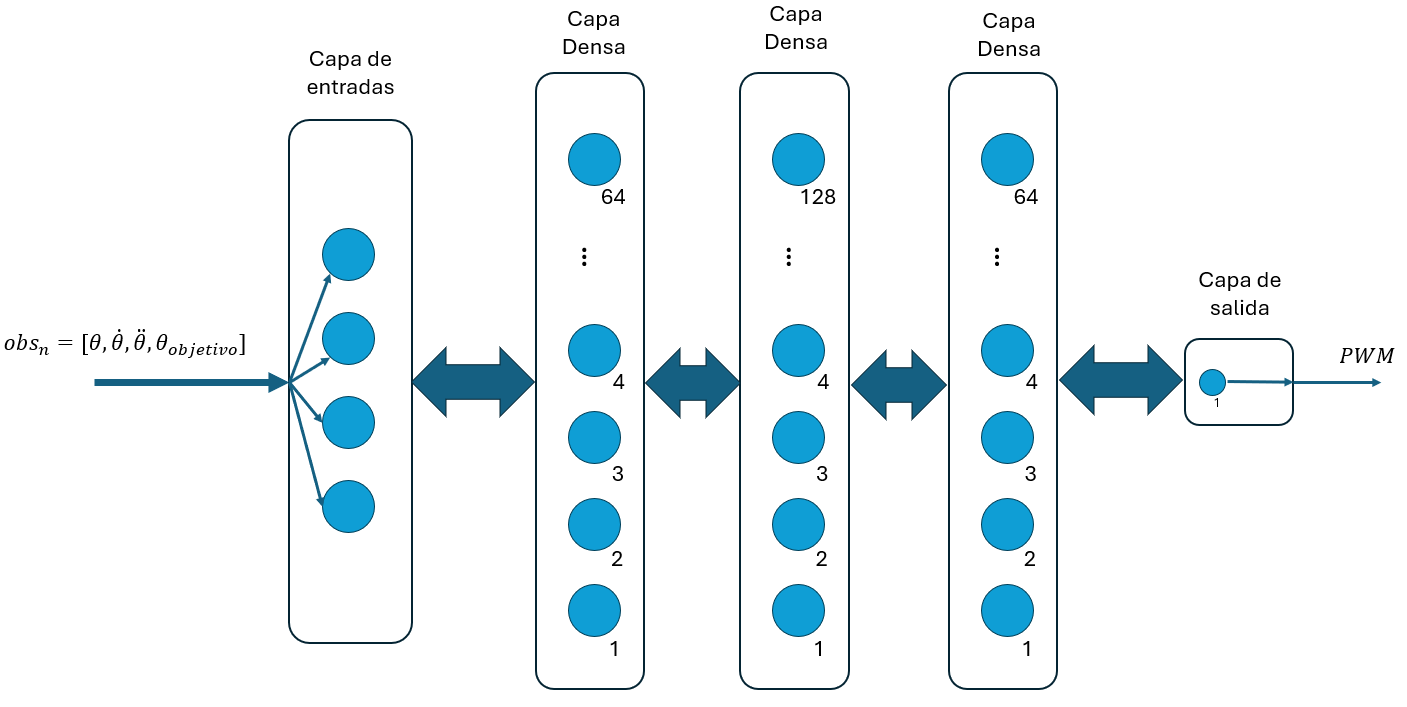
\includegraphics[scale=0.4]{fig/new/RNAPPO.png}
	\caption{Estructura de la RNA utilizada en el método PPO.}
	\label{fig:RNAparaPPO}
\end{figure}


\subsubsection{Plan de entrenamiento}

El algoritmo PPO base define su etapa de exploración con acciones aleatorias muestreadas a partir de una función de distribución normal centrada en la acción tomada por la RNA. En este caso se modificó el procedimiento para cumplir con las siguientes rutinas; se define una muestra de ruido de la distribución pero se fija su uso en una cantidad determinada de iteraciones, en un principio $10$, para ir diminuyendo una unidad cada doceava parte del tiempo de entrenamiento total, esto hasta mantener una muestra por iteración hacia el final del entrenamiento. Este cambio fue necesario para que el ruido agregado le permita al péndulo reaccionar, pues de otro modo la inercia del modelo elimina todo efecto de dicho ruido, que pretende forzar cierta exploración del espacio de estados.

Otra modificación propuesta es la disminución del valor de varianza inicial utilizado, $\sigma^2 = 0.01$ para crear la distribución normal que se muestrea en el punto anterior. La varianza disminuye con el mismo paso que la muestra estática mencionada, pero con una magnitud de $0.001$, esto hasta llegar a un valor mínimo del  $\sigma^2 = 0.001$.

Por último, en lugar de utilizar la muestra directa de la distribución como acción $a_t$, se considera como una muestra de ruido $n_t$ sumada con la señal $a_t$ de la RNA, de la siguiente manera:
\begin{equation}
a_{n} = a_t + n_t
\end{equation}
resultado al que se le limíta la respuesta respetando los valores de seguridad mencionados ($min=0$, $max=0.25$). Al resultado limitado $a'_{n}$ se le sustrae el $a_t$ y se le calcula la probabilidad de aparición del ruido $n'_t$ en la  distribución normal.

Todo los pasos anteriores ocurren durante las pruebas de observación al entorno y respuesta de la RNA, únicamente cambiando sus valores al cumplir el paso de una doceava parte del entrenamiento a la vez.


\subsection{Procesamiento y recopilación de datos}

En el presente proyecto se experimenta con los procesos de entrenamiento de modelos de RL para el control de la planta simulada PAMH, proceso que según se vió en la tabla \ref{tab:MatrizPugh}, requiere recursos computacionales considerables. Los entrenamientos y pruebas se realizaron en un computador con procesador Intel $i7-7700HQ$ de $2.80\, GHz$ con $8$ núcleos, con acceso a una unidad GPU de NVIDIA GeForce GTX $1050$ con $4\, GB$ de VRAM y mediante la herramienta \textit{Google Colab} de la empresa Google, utilizando \textit{Python 3 Google Compute Engine backend} con hasta $12\, GB$ de RAM y $108\, GB$ de almacenamiento.

Por otro lado, el protocolo de todos los procesos de entrenamiento realizados se concentran en la plataforma en línea \textit{Weights $\&$ Biases} (W$\&$B), servicio en línea orientado al aprendizaje automático.



\section{Evaluación de los modelos}

La evaluación del desempeño de los modelos se realiza con el promedio de la recompensa obtenida con el transcurso de los episodios en el entrenamiento de los modelos, donde se comparan diferentes resultados del promedio de la recompensa (diferentes entrenamientos) y se interpretan las aproximaciones a los valores más altos.

Luego de entrenado el modelo, se vuelve a montar el entorno con interfaz Gymnasium y se renderiza el comportamiento del PAMH en su versión virtual. En su segundo episodio se generan una curva de la respuesta angular del entorno respecto al tiempo, tomado directamente del sistema computacional. Con la curva de $\theta$ contra el tiempo en nanosegundos, se calcula el tiempo de subida, el tiempo de asentamiento y el sobreimpulso en la respuesta, esto procurando que el valor final del ángulo se encuentre en un rango de $\pm \, 10\%$ con diferencia al valor deseado $\theta_{objetivo}$.


